%导言区

\documentclass[10pt]{ctexart}%book,report,letter  10,11,12磅
\title{\heiti 我的 first document}
\author{meng jie}
\date{\today}
%\usepackage{ctex}%使用中文
\newcommand\degree{^\circ}
\newcommand{\myfont}{\textbf{\textsf{fancy text}}}
\usepackage{xltxtra}%XeLaTeX
\usepackage{amsmath}%equation*、matrix
\usepackage{amssymb}
\usepackage{graphicx}%eps,pdf,png,jpeg,bmp
\graphicspath{{figures/},{pics/}}
\newcommand\PRC{people 's republic of \emph{China}}%字符串替换
\newcommand\hateby[2]{#2 不受 #1 喜欢}
\newcommand\loves[2]{#1 喜欢 #2}
\newcommand\love[3][喜欢]{#2#1#3}
%正文区(文稿区)
\begin{document}
	\PRC
	
	\loves{猫儿}{鱼}
	
	\hateby{猫儿}{萝卜}
	
	\love{猫儿}{鱼}
	
	\love[最爱]{猫儿}{鱼}
	
	\section{多行公式排班}
	\begin{gather}
		a+b=b+a\notag \\%阻止编号
		ab ba
	\end{gather}
	
	\begin{gather*}
	a+b=b+a\\
	ab ba
	\end{gather*}
	
	\begin{align}%用&对齐
	a+b &=b+a\\
	ab  &= ba
	\end{align}
	
	\begin{align*}
	a+b&=b+a\\
	ab&= ba
	\end{align*}
	
	\begin{equation}
		\begin{split}
		\cos 2x&= \cos^2 x- \sin^2 x \\
		&= 2\cos^2 x - 1
		\end{split}
	\end{equation}
	
	\begin{equation}
		D(x)=\begin{cases}
		1,& \text{如果} x \in \mathbb{Q};\\
		0,& \text{如果} x \in \mathbb{R}\setminus\mathbb{Q};
		\end{cases}
	\end{equation}
	
	\section{矩阵}
	
	\[
	\begin{matrix}
		0 & 1 \\
		1 & 0 
	\end{matrix}
	\] \quad
	\[
	 \begin{pmatrix}
	 	0 & 1 \\
	 	1 & 0
	 \end{pmatrix}\quad\]
 	\[
 	\begin{bmatrix}
 		0 & 1 \\
 		1 & 0
 	\end{bmatrix}
 	\]
 	
 	\[
 	A= \begin{bmatrix}
 		a_{11} & \dots & a_{ln} \\
 		& \ddots & \vdots \\
 		0 & & a_{nn}
 	\end{bmatrix}_{n \times n}
	\]
	
	
	%分块矩阵
	\[
	\begin{pmatrix}
	\begin{matrix} 1&0 \\0&1 \end{matrix}
	& \text{\Large 0} \\
	\text{\Large 0} & \begin{matrix}
	1&0\\0&-1 
	\end{matrix}
	\end{pmatrix}
	\]
	
	%三角矩阵
	\[
	\begin{pmatrix}
		a_{11} & a_{12} & \cdots &a_{ln}\\
		&a_{22} & \cdots & a_{2n}\\
		&       &\ddots & \vdots \\
		\multicolumn{2}{c}{\raisetag{1.3ex}[0pt]{\Huge 0}}
		&       &a_{nn}
	\end{pmatrix}
	\]
	
	%跨列省略号
	\[
	\begin{pmatrix}
	1 & \frac 12 & \dots  & \frac ln \\
	\hdotsfor{4}\\
	m & \frac m2 & \dots & \frac mn
	\end{pmatrix}
	\]
	
	%行内小矩阵
	复数,也可以用矩阵
	\begin{math}
		\left(
		\begin{smallmatrix}
		x & -y \\ y & a
		\end{smallmatrix}
		\right)
	\end{math}
	
	%array环境
	\[
	\begin{array}{r|r}
	\frac12 & 0\\
	\hline
	0 & -\frac a{bc} \\
	\end{array}
	\]
	
	
	\section{数学公式}
	$1+2=2+1=3$
	
	\(1+2=2+1=3\)
	
	\begin{math}
		1+2=2+1=3
	\end{math}
	
	$3x^{20}+x-1=0$
	
	$3x^{3x^{20}+x-1=0}+x-1=0$
	
	$a_0,a_1,a_2,```$
	
	
	$\alpha$  $\beta$  $\gamma$  $\epsilon$  $\pi$  $\omega$  
	
	$\Gamma$  $\Delta$ $\Theta$  $\Pi$  $\Omega$
	
	$\sin$ $\cos$ $\log$  $\arcsin$  $\arccos$ $\ln$
	
	$\sqrt[4]{x^2 + y^2}$
	
	$\frac{3}{x^2 + y^2}$
	
	
	$$ \frac{3}{x^2 + y^2}  $$
	
	\[ 1+2=2+1=3\]
	\begin{displaymath}
		1+2=2+1=3
	\end{displaymath}
	
	\begin{equation}
		1+2=2+1=3\label{eq:commutative}
	\end{equation}
	
	\begin{equation*}
	1+2=2+1=3\label{eq:commutative2}
	\end{equation*}
	交换律见式\ref{eq:commutative},交换律见式\ref{eq:commutative2}%section 编号
	
	
	\begin{table}[h]
		\centering
		\caption{表格题注}\label{tab-score}
		\begin{tabular}{l | c |c| p{1.5cm}| r}
			\hline \hline
			姓名 & 语文 & 数学 & 外语 & 备注 \\
			\hline  \hline
			张三 & 87 & 100 & 96 &优秀\\
			\hline
			李四 & 87 & 100 & 96 &优秀\\
		\end{tabular}
	
	\end{table}
	
	\begin{figure}[htbp]
		
		\LaTeX{}中的插图:
		
		%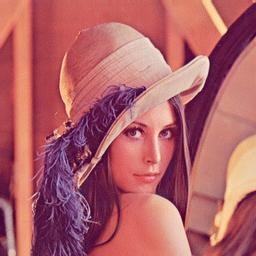
\includegraphics[angle=45,scale=0.3,height=0.1\textheight]{lena.jpeg}
		\caption{\TeX 图片题注} \label{fig-lena}
	\end{figure}
	
	图片见图\ref{fig-lena},表格见表\ref{tab-score}%交叉引用
	
	
	\maketitle
	
	hello world!
	

	
	let $f(x)$ be defined by the formal
	$$f(x)=3x^2+x-1$$ which is a polynomial of degree 2.
	
	$f(x)=3x^2+x-1$.
	你好,\LaTeXe 。  
	设直角三角形$ABC$,其中$\angle C=90\degree$,则有:
	\begin{equation}%产生带编号的行间公式
	AB^2=BC^2+AC^2.
	\end{equation}
	
	%字体族设置(罗马字体、无衬线字体、打字机字体)
	\textrm{roman family}     \textsf{sans serif family}    \texttt{typewriter family}
	
	{\rmfamily roman family}
	{\sffamily sans serif family}用{}可以限定范围
	{\ttfamily typewriter family}
	
	
	\rmfamily roman family
	
	%字体形状(直立、斜体、伪斜体、小型大写)
	\textup{upright shape}   \textit{italic shape}
	\textsl{slanted shape}   \textsc{small caps shape}
	
	{\upshape upright shape} {\itshape italic shape}
	{\slshape slanted shape} {\scshape caps shape}	
	
	%中文字体
	{\songti 宋体} \quad {\heiti 黑体} \quad {\fangsong 仿宋}  \quad {\kaishu 楷书}
	
	中文字体的\textbf{粗体}与\textit{斜体}
	
	%字体大小
	{\tiny  hello}\\
	{\scriptsize hello}\\
	{\footnotesize hello}\\
	{\small hello}\\
	{\normalsize hello}\\
	{\large hello}\\
	{\Large hello}\\
	{\LARGE hello}\\
	{\huge hello}\\
	{\Huge hello}\\
	
	%中文字号设置
	{\zihao{-0} 你好!}%-0 小初号
	
	\myfont 
	
	\section{空白符号}
	通过相机标定的程序获取了两个相机各自的内参矩阵和畸变系数,以及两个相机达到平行时各自的旋转矩阵。
	
	\par Opencv和Matlab都给了我们现成的函数,\quad 可以利用这些数据进行去畸变或者双目平行校正,\qquad Windows version 6.2 detected因为有需求要将去畸变和平行校正移植到硬件上,那么自己如何利用这些参数和矩阵写去畸变的程序和双目平行校正的程序呢?我本人发现的网上这方面资料较少。\par 在此总结一下。
	%\chapter{绪论}%ctexbook
	\section{\LaTeX 控制符}
	\# \$ \% \{ \} \~{} \textbackslash \&
	
	\section{排版符号}
	
	\subsection{\TeX 标志符号}
	\LaTeX{} \TeX{}  \LaTeXe{}
	\XeLaTeX
	\subsubsection{引号}
	` ' `` ''
	\subsection{连字符}
	- -- ---
	\section{非英文字符}
	\oe \OE \ae \AE \aa \AA \o \O  \l \L \ss \SS !` ?`
	\section{重度符号(以o为例)}
	\`o \'o \^o \''o \~o \.o \u{o} \v{o} \H{o} 
	\r{o} \t{o} \b{o} \c{o} \d{o}
	

	
	
\end{document}